% chap07 - Functions of vectors
% Last edited:

\chapter{Functions of vectors}


\section{Functions and files}
\label{funfiles}

So far we have only put one function in each file. It is also
possible to put more than one function in a file, but only the first
one, the {\bf top-level function} can be called from the Command
Window. The other {\bf helper functions} can be called from anywhere
inside the file, but not from any other file.

Large programs almost always require more than one function; keeping
all the functions in one file is convenient, but it makes debugging
difficult because you can't call helper functions from the Command
Window.

To help with this problem, I often use the top-level function
to develop and test my helper functions. For example, to write
a program for Exercise~\ref{duck}, I would create a file named
{\tt duck.m} and start with a top-level function named {\tt duck}
that takes no input variables and returns no output value.

Then I would write a function named {\tt error\_func} to
evaluate the error function for {\tt fzero}. To test
{\tt error\_func} I would call it from {\tt duck} and then
call {\tt duck} from the Command Window.

Here's what my first draft might look like:

\begin{verbatim}
function res = duck()
  error = error_func(10)
end

function res = error_func(h)
  rho = 0.3;   % density in g / cm^3
  r = 10;     % radius in cm
  res = h;
end
\end{verbatim}

The line {\tt res = h} isn't finished yet, but this
is enough code to test.
Once I finished and tested {\tt error\_func}, I would modify
{\tt duck} to use {\tt fzero}.

For this problem I might only need two functions, but if there
were more, I could write and test them one at a time, and then
combine them into a working program.



\section{Physical modeling}
\label{modeling}

Most of the examples so far have been about mathematics;
Exercise~\ref{duck}, the ``duck problem,'' is the first example we
have seen of a physical system. If you didn't work on this exercise,
you should at least go back and read it.

This book is supposed to be about {\bf physical modeling}, so it might
be a good idea to explain what that is. Physical modeling is a process
for making predictions about physical systems and explaining their
behavior. A {\bf physical system} is something in the real
world that we are interested in, like a duck.

The following figure shows the steps of this process:

\beforefig \centerline{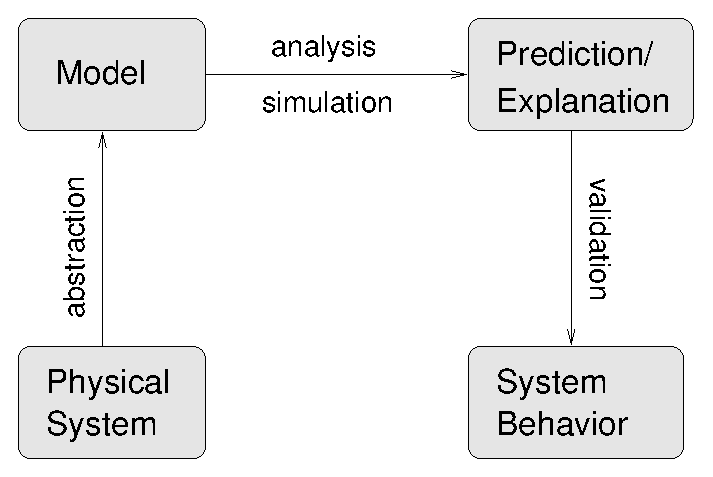
\includegraphics[height=1.5in]{figs/model.eps}}

A {\bf model} is a simplified description of a physical system. The
process of building a model is called {\bf abstraction}. In this
context, ``abstract'' is the opposite of ``realistic;'' an abstract
model bears little direct resemblance to the physical system it
models, in the same way that abstract art does not directly depict
objects in the real world. A realistic model is one that includes
more details and corresponds more directly to the real world.

Abstraction involves making justified decisions about which factors to
include in the model and which factors can be simplified or ignored.
For example, in the duck problem, we took into account the density of
the duck and the buoyancy of water, but we ignored the buoyancy of the
duck due to displacement of air and the dynamic effect of paddling
feet. We also simplified the geometry of the duck by assuming that
the underwater parts of a duck are similar to a segment of a sphere.
And we used coarse estimates of the size and weight of the duck.

Some of these decisions are justifiable. The density of the duck
is much higher than the density of air, so the effect of buoyancy
in air is probably small. Other decisions, like the spherical
geometry, are harder to justify, but very helpful. The actual
geometry of a duck is complicated; the sphere model makes it possible
to generate an approximate answer without making detailed measurements
of real ducks.

A more realistic model is not necessarily better. Models are useful
because they can be analyzed mathematically and simulated
computationally. Models that are too realistic might be difficult to
simulate and impossible to analyze.

A model is successful if it is good enough for its purpose. If we
only need a rough idea of the fraction of a duck that lies below
the surface, the sphere model is good enough. If we need a more
precise answer (for some reason) we might need a more realistic
model.

% Einstein's actual quote: ``It can scarcely be denied that the supreme
% goal of all theory is to make the irreducible basic elements as simple
% and as few as possible without having to surrender the adequate
% representation of a single datum of experience.

%   * "On the Method of Theoretical Physics" The Herbert Spencer
%    Lecture, delivered at Oxford (10 June 1933); also published in
%    Philosophy of Science, Vol. 1, No. 2 (April 1934),
%    pp. 163-169. [thanks to Dr. Techie @ www.wordorigins.org and
%    JSTOR]

Checking whether a model is good enough is called {\bf validation}.
The strongest form of validation is to make a measurement of an
actual physical system and compare it to the prediction of a
model.

If that is infeasible, there are weaker forms of validation. One is
to compare multiple models of the same system. If they are
inconsistent, that is an indication that (at least) one of them is
wrong, and the size of the discrepancy is a hint about the reliability
of their predictions.

We have only seen one physical model so far, so parts of this
discussion may not be clear yet. We will come back to these topics
later, but first we should learn more about vectors.



\section{Vectors as input variables}

Since many of the built-in functions take vectors as arguments,
it should come as no surprise that you can write functions that
take vectors. Here's a simple (silly) example:

\begin{verbatim}
function res = display_vector(X)
  X
end
\end{verbatim}

There's nothing special about this function at all. The only
difference from the scalar functions we've seen is that I used
a capital letter to remind me that {\tt X} is a vector.

This is another example of a function that doesn't actually have
a return value; it just displays the value of the input variable:

\begin{verbatim}
octave:1> display_vector(1:3)
X = 1   2   3
\end{verbatim}

Here's a more interesting example that encapsulates the code
from Section~\ref{reduce} that adds up the elements of a vector:

\begin{verbatim}
function res = mysum(X)
  total = 0;
  for i=1:length(X)
    total = total + X(i);
  end
  res = total;
end
\end{verbatim}

I called it {\tt mysum} to avoid a collision with the built-in
function {\tt sum}, which does pretty much the same thing.

Here's how you call it from the Command Window:

\begin{verbatim}
octave:2> total = mysum(1:3)
total = 6
\end{verbatim}

Because this function has a return value, I made a
point of assigning it to a variable.


\section{Vectors as output variables}

There's also nothing wrong with assigning a vector to an output
variable. Here's an example that encapsulates the code from
Section~\ref{apply}:

\begin{verbatim}
function res = myapply(X)
  for i=1:length(X)
    Y(i) = X(i)^2
  end
  res = Y
end
\end{verbatim}

Ideally I would have changed the name of the output variable to
{\tt Res}, as a reminder that it is supposed to get a vector value,
but I didn't.

Here's how {\tt myapply} works:

\begin{verbatim}
octave:1> V = myapply(1:3)
V = 1   4   9
\end{verbatim}

\begin{ex}
Write a function named {\tt find\_target} that
encapsulates the code, from Section~\ref{search}, that finds the
location of a target value in a vector.
\end{ex}


\section{Vectorizing your functions}

Functions that work on vectors will almost always work on scalars
as well, because Octave considers a scalar to be a vector with
length 1.

\begin{verbatim}
octave:1> mysum(17)
ans = 17

octave:2> myapply(9)
ans = 81
\end{verbatim}

Unfortunately, the converse is not always true. If you write
a function with scalar inputs in mind, it might not work on vectors.

But it might! If the operators and functions
you use in the body of your function work on vectors, then your
function will probably work on vectors.

For example, here is the very first function we wrote:

\begin{verbatim}
function res = myfunc (x)
  s = sin(x)
  c = cos(x)
  res = abs(s) + abs(c)
end
\end{verbatim}

And lo! It turns out to work on vectors:

\begin{verbatim}
octave:3> Y = myfunc(1:3)
Y = 1.3818  1.3254  1.1311
\end{verbatim}

At this point, I want to take a minute to acknowledge that I
have been a little harsh in my presentation of Octave, because
there are a number of features that I think make life harder
than it needs to be for beginners. But here, finally,
we are seeing features that show Octave's strengths.

Some of the other functions we wrote don't work on vectors,
but they can be patched up with just a little effort. For example,
here's {\tt hypotenuse} from Section~\ref{hypotenuse}:

\begin{verbatim}
function res = hypotenuse(a, b)
  res = sqrt(a^2 + b^2);
end
\end{verbatim}

This doesn't work on vectors because the \verb+^+ operator
tries to do matrix exponentiation, which only works on
square matrices.

\begin{verbatim}
octave:1> hypotenuse(1:3, 1:3)
??? Error using ==> mpower
Matrix must be square.
\end{verbatim}

But if you replace \verb+^+ with the elementwise operator
\verb+.^+, it works!

\begin{verbatim}
octave:1> A = [3,5,8];
octave:1> B = [4,12,15];
octave:1> C = hypotenuse(A, B)

C = 5  13  17
\end{verbatim}
 
In this case, it matches up corresponding elements from the two
input vectors, so the elements of {\tt C} are the hypotenuses of
the pairs $(3,4)$, $(5,12)$ and $(8,15)$, respectively.

In general, if you write a function using only elementwise
operators and functions that work on vectors, then the new
function will also work on vectors.


\section{Sums and differences}

Another common vector operation is {\bf cumulative sum}, which takes a
vector as an input and computes a new vector that contains all of the
partial sums of the original. In math notation, if $V$ is the
original vector, then the elements of the cumulative sum, $C$, are:

\[ C_i = \sum_{j=1}^i V_j \]

In other words, the $i$th element of $C$ is the sum of the first
$i$ elements from $V$. Octave provides a function named {\tt cumsum}
that computes cumulative sums:

\begin{verbatim}
octave:1> V = 1:5
V = 1   2   3   4   5

octave:2> C = cumsum(V)
C = 1   3   6  10  15
\end{verbatim}

\begin{ex}
Write a function named {\tt cumulative\_sum} that uses
a loop to compute the cumulative sum of the input vector.
\end{ex}

The inverse operation of {\tt cumsum} is {\tt diff}, which computes
the difference between successive elements of the input vector.

\begin{verbatim}
octave:3> D = diff(C)
D = 2   3   4   5
\end{verbatim}

Notice that the output vector is shorter by one than the input
vector. As a result, Octave's version of {\tt diff} is not
exactly the inverse of {\tt cumsum}. If it were, then we would
expect {\tt cumsum(diff(X))} to be {\tt X}:

\begin{verbatim}
octave:4> cumsum(diff(V))
ans = 1   2   3   4
\end{verbatim}

But it isn't.

\begin{ex}
Write a function named {\tt mydiff} that computes the
inverse of {\tt cumsum}, so that {\tt cumsum(mydiff(X))} and
{\tt mydiff(cumsum(X))} both
return {\tt X}.
\end{ex}


\section{Products and ratios}

The multiplicative version of {\tt cumsum} is {\tt cumprod},
which computes the {\bf cumulative product}. In math notation,
that's:

\[ P_i = \prod_{j=1}^i V_j \]

In Octave, that looks like:

\begin{verbatim}
octave:1> V = 1:5
V = 1   2   3   4   5

octave:2> P = cumprod(V)
P = 1   2   6  24  120
\end{verbatim}

\begin{ex}
Write a function named {\tt cumulative\_prod} that uses
a loop to compute the cumulative product of the input vector.
\end{ex}

Octave doesn't provide the multiplicative version
of {\tt diff}, which would be called {\tt ratio}, and which would
compute the ratio of successive elements of the input vector.

\begin{ex}
Write a function named {\tt myratio} that computes the
inverse of {\tt cumprod}, so that {\tt cumprod(myratio(X))} and
{\tt myratio(cumprod(X))} both
return {\tt X}.

You can use a loop, or if you want to be clever, you can take
advantage of the fact that $e^{\ln a + \ln b} = a b$.

If you apply {\tt myratio} to a vector that contains Fibonacci
numbers, you can confirm that the ratio of successive elements
converges on the golden ratio, $(1+\sqrt{5})/2$ (see
Exercise~\ref{fibratio}).
\end{ex}



\section{Existential quantification}

It is often useful to check the elements of a vector to see if there
are any that satisfy a condition. For example, you might want to
know if there are any positive elements. In logic, this condition
is called {\bf existential quantification}, and it is denoted with
the symbol $\exists$, which is pronounced ``there exists.'' For example,
this expression

\[ \exists x \mbox{~in~} S: x>0 \]

means, ``there exists some element $x$ in the set $S$ such that
$x>0$.'' In Octave it is natural to express this idea with a logical
function, like {\tt exists}, that returns 1 if there is such an
element and 0 if there is not.

\begin{verbatim}
function res = exists(X)
  for i=1:length(X)
    if X(i) > 0
      res = 1;
      return
    end
  end
  res = 0;
end
\end{verbatim}

We haven't seen the {\tt return} statement before; it is similar
to {\tt break} except that it breaks out of the whole function, not
just the loop. That behavior is what we want here because as soon
as we find a positive element, we know the answer (it exists!) and
we can end the function immediately without looking at the rest
of the elements.

If we exit at the end of the loop, that means we didn't find what
we were looking for (because if we had, we would have hit the
{\tt return} statement).



\section{Universal quantification}

Another common operation on vectors is to check whether {\em all}
of the elements satisfy a condition, which is known to
logicians as {\bf universal quantification} and denoted with
the symbol $\forall$ which is pronounced ``for all.'' So this
expression

\[ \forall x \mbox{~in~} S: x>0 \]

means ``for all elements, $x$, in the set $S$, $x>0$.''

A slightly silly way to evaluate this expression in Octave is to
count the number of elements that satisfy the condition.
A better way is to reduce the problem to
existential quantification; that is, to rewrite

\[ \forall x \mbox{~in~} S: x>0 \]

as

\[ \sim \exists x \mbox{~in~} S: x \le 0 \]

Where $\sim \exists$ means ``does not exist.''
In other words, checking that all the elements are positive is
the same as checking that there are no elements 
that are non-positive.

\begin{ex}
Write a function named {\tt forall} that
takes a vector and returns 1 if all of the elements are positive
and 0 if there are any non-positive elements.
\end{ex}




\section{Logical vectors}

When you apply a logical operator to a vector, the result is a {\bf
logical vector}; that is, a vector whose elements are the logical
values 1 and 0.

\begin{verbatim}
octave:1> V = -3:3
V = -3  -2  -1   0   1   2   3

octave:2> L = V>0
L = 0   0   0   0   1   1   1
\end{verbatim}

In this example, {\tt L} is a logical vector whose elements
correspond to the elements of {\tt V}. For each positive element of
{\tt V}, the corresponding element of {\tt L} is 1.

Logical vectors can be used like flags to store the state of
a condition. They are also often used with the {\tt find} function,
which takes a logical vector and returns a vector that contains
the indices of the elements that are ``true.''

Applying {\tt find} to {\tt L} yields

\begin{verbatim}
octave:3> find(L)
ans = 5   6   7
\end{verbatim}

which indicates that elements 5, 6 and 7 have the value 1.

If there are no ``true'' elements, the result is an empty vector.

\begin{verbatim}
octave:4> find(V>10)
ans = [](1x0)
\end{verbatim}

This example computes the logical vector and passes it as an
argument to {\tt find} without assigning it to an intermediate
variable. You can read this version abstractly as ``find
the indices of elements of {\tt V} that are greater than 10.''

We can also use {\tt find} to write {\tt exists} more concisely:

\begin{verbatim}
function res = exists(X)
  L = find(X>0)
  res = length(L) > 0
end
\end{verbatim}

\begin{ex}
Write a version of {\tt forall} using {\tt find}.
\end{ex}


\section{Glossary}

\begin{description}

\item[top-level function:] The first function in an M-file;
it is the only function that can be called from the Command
Window or from another file.

\item[helper function:] A function in an M-file that is not
the top-level function; it only be called from another function
in the same file.

\item[physical modeling:] A process
for making predictions about physical systems and explaining their
behavior.

\item[physical system:] Something in the real world that we are
interested in studying.

\item[model :] A simplified description of a
physical system that lends itself to analysis or simulation.

\item[abstraction:] The process of building a model by making
decisions about what factors to simplify or ignore.

\item[validation:] Checking whether a model is adequate for its
purpose.

\item[existential quantification:] A logical condition that expresses
the idea that ``there exists'' an element of a set with a certain
property.

\item[universal quantification:] A logical condition that expresses
the idea that all elements of a set have a certain property.

\item[logical vector:] A vector, usually the result of applying a logical
operator to a vector, that contains logical values 1 and 0. 


\end{description}

%\section{Exercises}

%\begin{ex}
%\end{ex}
